% !TEX root = ../ac_paper.tex

\section{Classical search algorithms}\label{sec:search}

In this section, we compare the effectiveness of breadth-first and greedy search algorithms to AC-trivialize presentations in the Miller--Schupp series.
We find that the latter significantly outperforms the former. Based on our empirical observations, we find AC-triviality of infinite subfamilies of the Miller--Schupp series, as well as length reductions of $\AK(n)$. 

\subsection{Breadth-first search}

In breadth-first search (See \cref{alg:bfs} for pseudocode), we start with an initial state, which is a balanced presentation we aim to AC-trivialize, and place it in a queue. At each iteration, a state is removed from the queue, and its neighbors are added if they have not already been visited. This process continues until the sought-after state, i.e., a trivial balanced presentation, is found or a maximum number of states $N$ is visited. In our experiments, we set $N = 10^6$.

\begin{algorithm}
	\caption{Breadth-First Search}\label{alg:bfs}
	\begin{algorithmic}[1] % The number [1] ensures lines are numbered
		\State \textbf{Input:} A balanced presentation $\pi$, maximum number of states to visit $N$
		\State \textbf{Output:} Boolean for whether an AC trivialization is found
		\State Initialize a queue $Q$ and enqueue the starting node $\pi$
		\State Mark $\pi$ as visited
		\While{Number of visited states is less than $N$}
		\State $u \gets Q$.dequeue() \Comment{Remove the front node of $Q$}
		\For{each neighbor $v$ of $u$}
		\If{$v$ is a trivial state}
		\State \Return True \Comment{Return True if $v$ is a trivial state}
		\EndIf
		\If{$v$ has not been visited}
		\State Mark $v$ as visited
		\State $Q$.enqueue($v$) \Comment{Add $v$ to the queue}
		\EndIf
		\EndFor
		\EndWhile
		\State \Return False \Comment{Return False if no trivial state is found}
	\end{algorithmic}
\end{algorithm}

\subsection{Greedy search}\label{ss:greedy_search}

Greedy search, described in \cref{alg:gs}, differs only slightly from breadth-first search. We replace the queue with a priority queue, which stores the states in order determined by a tuple of values $(k, l)$, where $k$ is the length of the presentation and $l$ is the path length between the state and the initial state.

Instead of dequeuing the earliest state, the algorithm dequeues the state with the smallest value of $k$. If there is more than one state in the priority queue with the same value of $k$, the state with the smallest value of $l$ is chosen.

\begin{algorithm}
	\caption{Greedy Search}\label{alg:gs}
	\begin{algorithmic}[1] % The number [1] ensures lines are numbered
		\State \textbf{Input:} A balanced presentation $\pi$ of length $k$, maximum number of states to visit $N$
		\State \textbf{Output:} Boolean for whether an AC trivialization is found
		\State Initialize a \textit{priority} queue $Q$ ordered by $(k, l)$ and enqueue the starting node $\pi$.
		$l$ is the length of the path connecting $\pi$ to the current node.
		\State Mark $\pi$ as visited
		\While{Number of visited states is less than $N$}
		\State $u \gets Q$.dequeue() \Comment{Remove the front node of $Q$}
		\For{each neighbor $v$ of $u$}
		\If{$v$ is a trivial state}
		\State \Return True \Comment{Return True if $v$ is a trivial state}
		\EndIf
		\If{$v$ has not been visited}
		\State Mark $v$ as visited
		\State $Q$.enqueue($v$) \Comment{Add $v$ to the queue}
		\EndIf
		\EndFor
		\EndWhile
		\State \Return False \Comment{Return False if no trivial state is found}
	\end{algorithmic}
\end{algorithm}

\subsection{Comparison of performance on Miller--Schupp series}\label{sec:search-ms}

We find that greedy-search outperforms breadth-first search in the task of AC-trivializing Miller--Schupp presentations. %\cref{fig:performance}
Out of the 1190 presentations in the Miller--Schupp series with $n \leq 7$ and $\length(w) \leq 7$, greedy search solved 533 while BFS solved only 278.
Each algorithm was constrained to visit a maximum of 1 million nodes.
The percentage of presentations solved by these algorithms decreases monotonically as a function of $n$, with greedy search being able to solve all presentations with $n=1$ (see \cref{fig:performance_of_search_vs_n}).
This empirical result encouraged us to prove AC-triviality of the infinite family $MS(1, w)$, which we give in \cref{sec:ms1w_}.

\begin{figure}
	\centering
    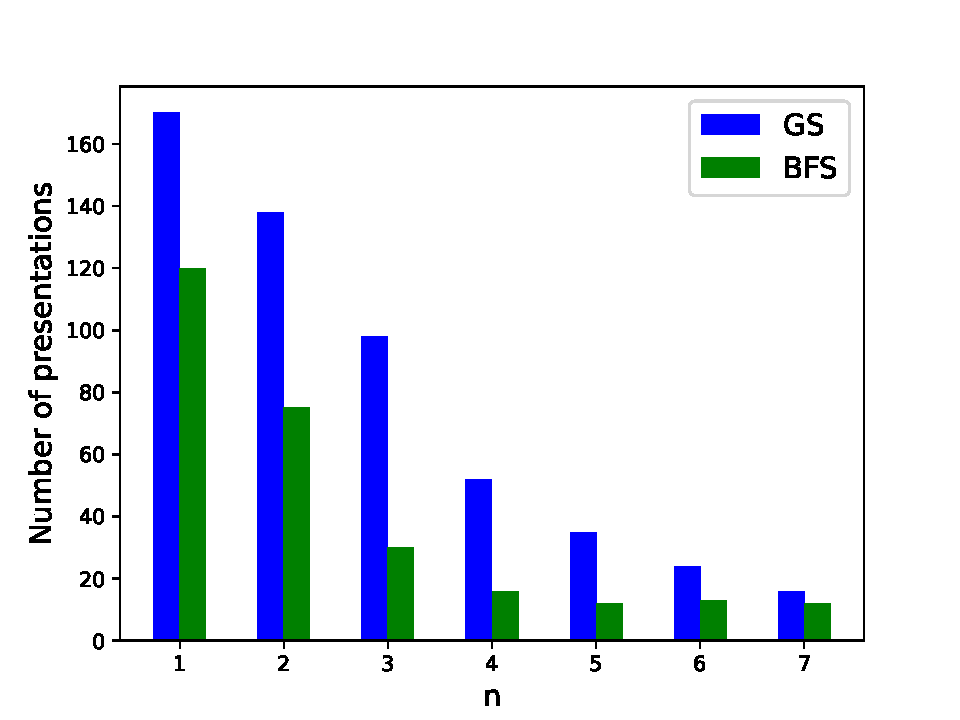
\includegraphics[width=0.6\textwidth]{fig/performance_of_search_vs_n.pdf}
    \caption{Comparison of greedy and breadth-first search algorithms as a function of $n$.
    The number of presentations of the Miller--Schupp series, $\MS(n, w)$, solved by an algorithm is given on the vertical axis.}
	\label{fig:performance_of_search_vs_n}
\end{figure}

Greedy search was also able to solve all presentations of length less than 14.
At length 14, there are six presentations that greedy search could not solve. We verified that four of these,
\[
\angles{x, y \mid x^{-1} y^2 x = y^{3} , x = x^{-2} y^{-1} x^2 y^{\pm 1}}
\]
\[
\angles{x, y \mid x^{-1} y^3 x = y^{4} , x = y^{\pm 1} x^2 y^{\pm 1}}
\]
are AC-equivalent to $\AK(3)$, while the other two
\[
\angles{x, y \mid x^{-1} y^2 x = y^{3} , x = y x^2 y^{\pm 1} x^{-2}}
\]
could be related neither to $\AK(3)$ nor to the trivial presentation through any path involving only presentations with both relators having length less than 20.

For presentations solved by greedy search, we plot the maximum amount by which the length of a presentation increased in an AC trivialization path in \cref{fig:gs_length_increase}.
In most cases, there was no increase in length; and the maximum increase was only~5.
At first glance, this seemed surprising to us, given that we allowed the relator lengths to increase by a much larger amount in our search process.\footnote{The length of each relator was allowed to increase up to \(2 \times \text{max}(2n+3, \length(w)+1) + 2\), which is twice the maximum of the initial lengths of the two relators in a presentation, plus an additional 2.
The maximum possible increase in presentation length is twice this number minus the original length.
For $n \leq 7$ and $\length(w) \leq 7$, this value lies in the range $[17, 53]$.}
However, the hard cutoff set by visiting a maximum of only 1 million nodes ensures that any presentation that needs to be mapped to a much longer presentation before it is trivialized would remain unsolved by the greedy search algorithm.
This limitation could be cured either by increasing the number of maximum nodes (at the cost of higher memory use) or by using a different criterion to order nodes in the priority queue.
It will be useful to explore the latter approach perhaps by looking for a criterion itself using deep learning algorithms.

We also plot the lengths of AC sequences discovered by greedy search as functions of $n$ and the maximum increase in the presentation length (\cref{fig:gs_path_length}).
Unsurprisingly, path lengths increase proportionally with the increase in the length of the presentation (\cref{fig:path_lengths_vs_length_increase}).
The following presentation with $n=5$ had the longest AC trivialization path,
\[
\angles{x, y \mid x^{-1} y^5 x = y^6,  x = y x^2 y^{-1}}
\] %correcting : \[\angles{x^{-1} y^5 x = y^6 \mid x = y x^2 y^{-1}}\]
requiring a sequence of 344 AC-moves.
Note that greedy search does not necessarily find the shortest paths of trivialization.
We will see in \cref{sec:application} that a Reinforcement Learning algorithm finds shorter trivializing sequences for many examples of the Miller--Schupp series.
This again hints at the potential utility of exploring more efficient criteria for ordering nodes in the priority queue.

In the remainder of this paper, we will refer to the presentations from the Miller--Schupp series that were solved and unsolved by the greedy search as ``GS-solved" and ``GS-unsolved" presentations, respectively. In other words, many of our experiments will be tested on two datasets that consists of Miller--Schupp presentations with $n \leq 7$ and $\length(w) \leq 7$: the GS-solved dataset has 533 presentations, whereas GS-unsolved dataset has 657 presentations. The combined dataset that contains all presentations with $n \leq 7$ and $\length(w) \leq 7$ has size 1190.

\begin{figure}
	\centering
	\begin{subfigure}[b]{0.5\textwidth}
		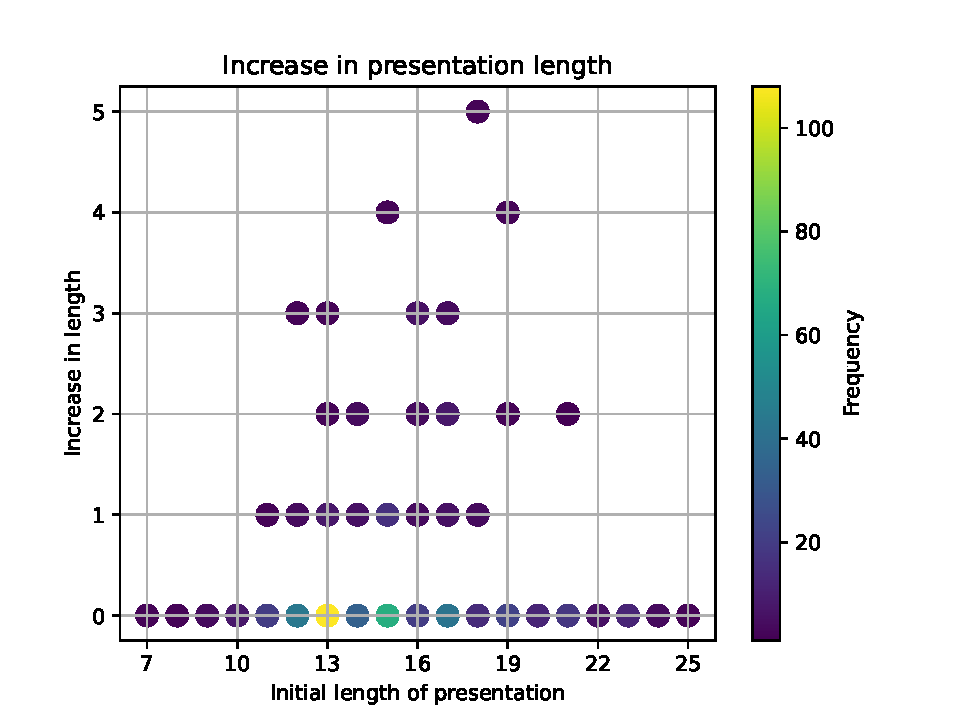
\includegraphics[width=\textwidth]{fig/gs_length_increase_vs_length.pdf}
		\caption{Distribution versus initial presentation length.}
		\label{fig:gs_length_increase_vs_length}
	\end{subfigure}%
	%add desired spacing between images, e. g. ~, \quad, \qquad etc.
	%(or a blank line to force the subfigure onto a new line)
	\begin{subfigure}[b]{0.5\textwidth}
		\centering
		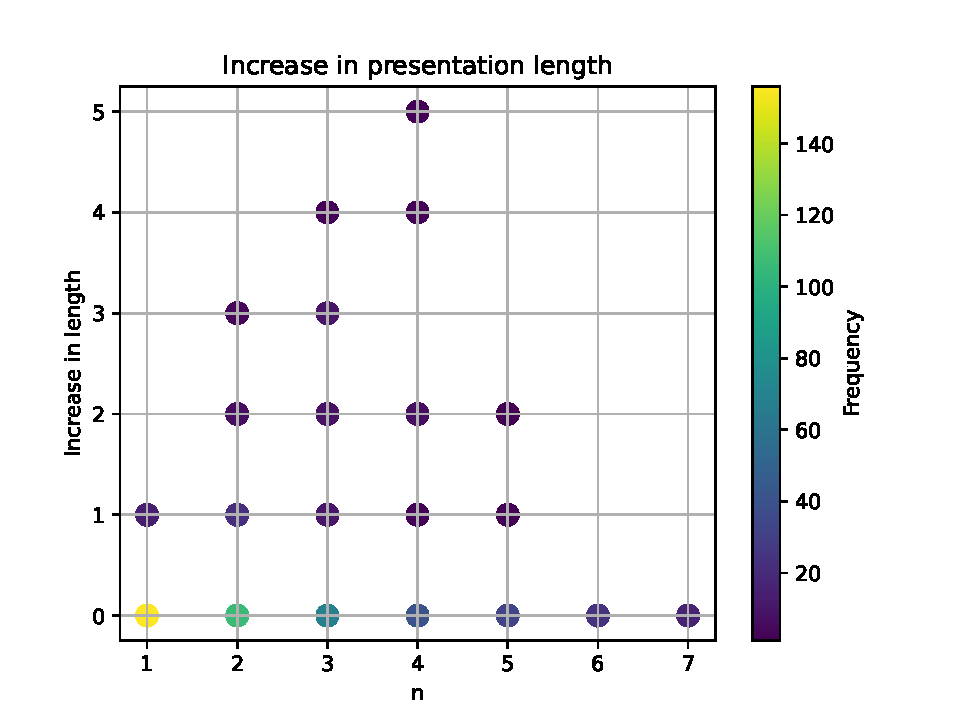
\includegraphics[width=1.1\textwidth]{fig/gs_length_increase_vs_n.pdf}
		\caption{Distribution versus $n$.}
		\label{fig:gs_length_increase_vs_n}
	\end{subfigure}
	\caption{The maximum increase in the length of a presentation relative to its initial length along the AC trivialization path. The increase is plotted as a function of the initial length of the presentation on the left and as a function of $n$ on the right.} \label{fig:gs_length_increase}
\end{figure}

\begin{figure}
	\centering
	\begin{subfigure}[b]{0.4\textwidth}
		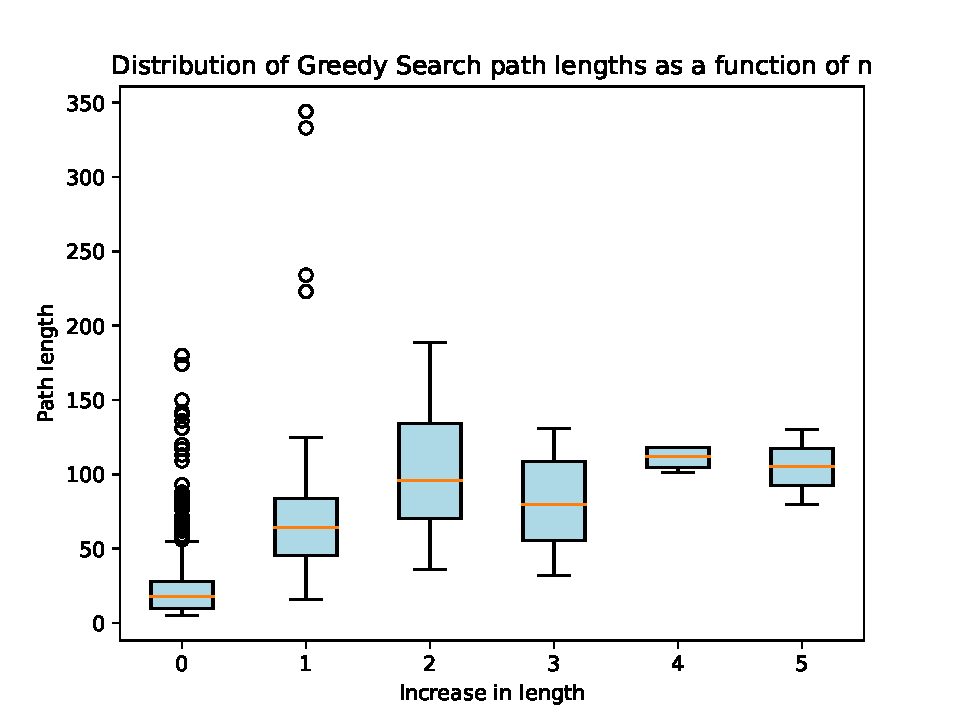
\includegraphics[width=\textwidth]{fig/path_lengths_vs_length_increase.pdf}
		\caption{Distribution versus maximum increase in presentation length.}
		\label{fig:path_lengths_vs_length_increase}
	\end{subfigure}
	\begin{subfigure}[b]{0.4\textwidth}
		\centering
		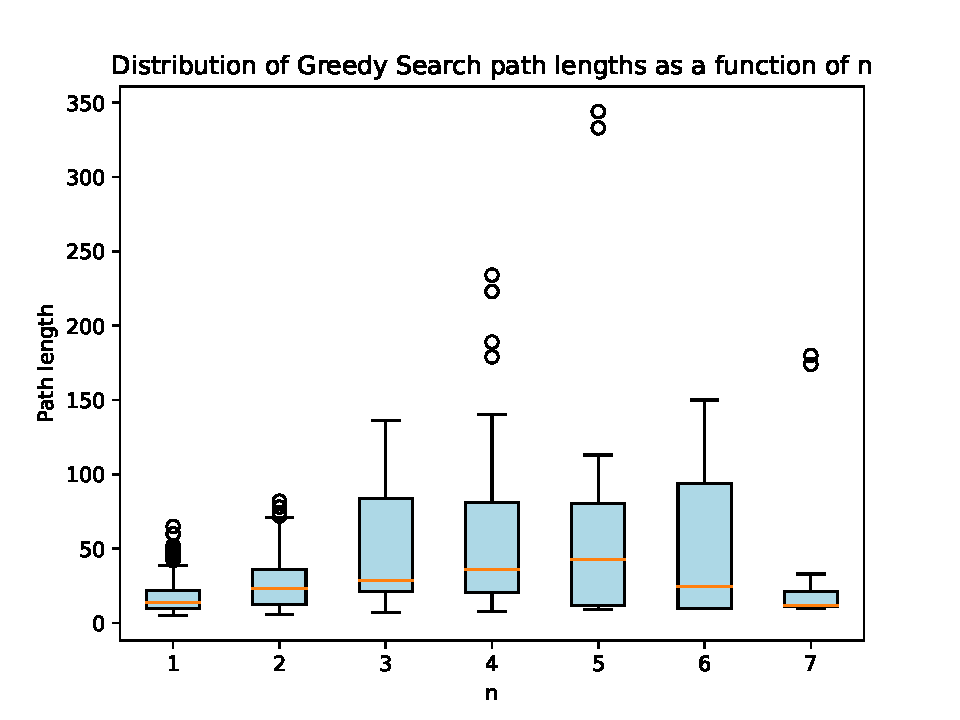
\includegraphics[width=1.1\textwidth]{fig/gs_path_lengths.pdf}
		\caption{Distribution versus $n$.}
		\label{fig:gs_path_lengths}
	\end{subfigure}%
	\caption{Distribution of lengths of AC-trivialization paths learned by greedy search as a function of maximum increase in presentation length (left) and $n$ (right).} \label{fig:gs_path_length}
\end{figure}

\subsection{AC-triviality of $\MS(1, w)$} \label{sec:ms1w_}

As mentioned in the previous subsection, the greedy search could solve all $n=1$ presentations of the Miller--Schupp series in our dataset. This motivated us to prove AC-triviality for all $\MS(1, w)$. 

In this and the following subsections, we frequently use the \emph{substitution} transformation mentioned in Section~\ref{sec:AC}.   

% The proof of this result, along with the results we present in the next section, relies on the substitution principle: \todo{Shehper: I am confused about how to present the substitution principle. 1. Should we skip Burns-Macedonska result and just mention the principle as we use it? This is exhibited in the example that follows. 2. Should we mention the substitution principle in Section 2 instead of here, right after we describe AC moves? 3. In section 8, we describe a substitution principle of stable AC conjecture. The first line of that proof is essentially what we need in this section. Should we refer our vanilla AC substitution lemma in the proof of that lemma?}

% \begin{lemma}[Burns, Macedonska, \cite{BurnsI}]\label{l:BM}
%     Let $P = \angles{x_1, \cdots, x_n \mid r_1, \cdots, r_n}$ be a presentation of the trivial group. $P$ is AC-equivalent to the presentation $\angles{x_1, \cdots, x_n \mid r_1, \cdots, r_{i-1}, r'_i, r_{i+1}, \cdots, r_n}$ where $r'_i$ is congruent to $r_i$ modulo the normal closure of  $\{r_1, \cdots, r_{i-1}, r_{i+1}, \cdots, r_n\}$.
% \end{lemma}

% \lucas{if I understand correctly, the lemma is also a consequence of the example that follows. I think it might be better for non-mathematical readers to present it in that language, espeically given that's how we use it. And then @Shehper I agree we should cite it in the stable section. But my overall preference would be to not state this as a lemma and just mention it when we use it} A simple consequence of this lemma is that we may substitute one relation into others. As an example, consider the presentation $\angles{x, y \mid xy = y^2 x, u x y v = e}$ where $u$ and $v$ are some words in $x$ and $y$. We will show that it is AC-equivalent to the presentation $\angles{x, y \mid xy = y^2 x, u y^2 x v}$ obtained by substituting the first relator into the second. First, use conjugation by $v$ to write the second relator as $vuxy$. Next, write the first relator as $(xy)^{-1} y^2 x$, and multiply the second relator by it. We get $vuy^2 x$, which we may conjugate by $v^{-1}$ to get the required result. 

\begin{theorem}\label{t:ms1wt}
    $\MS(1,w)$ is AC-trivial for all $w$.
\end{theorem}

\begin{proof}
We have 
\[
\MS(1, w) = \angles{x, y \mid x^{-1} y x = y^{2}, x = w}
\]
where $w$ has exponent sum 0 in $x$. We can re-write the first relator in the following four ways: 
\begin{enumerate}[label=(\roman*)]
    \item $yx=xy^2$
    \item $x^{-1}y = y^2 x^{-1}$
    \item $x^{-1}y^{-1}=y^{-2}x^{-1}$
    \item $y^{-1}x = xy^{-2}$
\end{enumerate}

We can substitute these equations in the second relator to move around all occurrences of $x$ and $x^{-1}$: relations (i) and (iv) move $x$ to the left, relations (ii) and (iii) move $x^{-1}$ to the right. We continue until the second relator becomes $x^{a-1} y^b x^{-a}$ for some $a, b \in \mathbb{Z}$. Through conjugation, this simplifies to $x = y^b$, which when substituted into the first relator leads to a trivialization of the presentation.
\end{proof}

The following result follows from this theorem.

\begin{theorem}\label{t:msnw}
    $\MS(n, w_\star)$ for $w_\star = y^{-1} x y x^{-1}$ is AC-trivial for all $n$.
\end{theorem}

\begin{proof}
In the presentation,
\[
\MS(n, w_\star) = \angles{x, y \mid x^{-1} y^n x = y^{n+1}, x = y^{-1} x y x^{-1} }
\]
we can rewrite the second relation as $y^{-1} x y = x^2$, and apply the automorphism $x \leftrightarrow y$ to get
\[
\MS(n, w_\star) = \angles{x, y \mid
x^{-1} y x = y^2 , y^{-1} x^n y = x^{n+1}}.
\]
This presentation is the same as $MS(1, y^{-1} x^n y x^{-n})$, which is AC-trivial by \cref{t:ms1wt}. 
\end{proof}

AC-trivializations of $MS(n, w_\star)$ for $n = 3, 4, 5, 6, 7, 8$ were recently obtained using automated theorem proving in \cite{new-ac-for-ms}. Here, we have obtained AC-trivializations of this family for all $n$.


% Indeed, to see how to realize this with AC moves, consider by means of example the application of (1) to $w_1yxw_2$. First, we cycle the relator to get $yxw_2w_1$, then invert it to get $w_1^{-1}w_2^{-1}x^{-1}y^{-1}$, and then multiply by (1) written as $yxy^{-2}x^{-1}$ onto the end of the relator, giving $w_1^{-1}w_2^{-2}y^{-2}x^{-1}$. Inverting again and cycling gives us $w_1xy^2w_2$. 

% After moving all positive powers of $x$ to the left and negative powers of $x$ to the right, we can cancel them with (AC3) by conjugating by $x^{-1}$. We are then left with $y^kx^{-1}$ for some $k$, since the exponent sum on $x$ in the second relator was $-1$ to begin with and is unchanged throughout these moves. Substituting this into the first relation, we get $y=y^2$ or $y=1$, from which we can easily trivialize the second relator as well. 


\subsection{Length reduction for $\AK(n)$}
\label{sec:len-reduction}

In \cref{sec:search-ms}, we discussed the performance of classical search algorithms for presentations of the Miller--Schupp series. But what if we apply these algorithms for presentations of the Akbulut--Kirby series instead? We find that starting from $AK(5)$---a presentation of length $17$---and performing greedy search for $20$ million nodes, reduces its length to 16. Examining the sequence of AC moves connecting the two presentations, we found the following result.\shehper{@Anibal, all: Two paper-wide issues to mention here: 1. Should we try to match numbering of theorems in introduction with their numbering in later sections, and 2. when we autoref lemma or proposition, it is referenced as a Theorem instead. I dont know how to fix that..}

\begin{theorem}\label{t:n+11}
	For every $n\geq 2$, $\AK(n)$ is AC-equivalent to the presentation
	\[
	\angles{ x,y \mid x^{-1} y x = x y x^{-1} y \ ,\  xyx=yx^{n-1}y },
	\]
	of length $n+11$. This gives reduction in length of $AK(n)$ for all $n \geq 5$.
\end{theorem}

To prove this theorem, we will  use the following result due to \cite{MMS}, and prove two additional theorems (\cref{t:mswk_wk1} and \cref{t:ms-short}). From these results, \cref{t:n+11} follows immediately. 

\begin{proposition}
    [Myasnikov, Myasnikov, and Shpilrain, \cite{MMS}]\label{t:MS-AK-MS}
    For all $n \geq 2$, $AK(n)$ is AC-equivalent to $MS(n, w_1)$ where $w_1 = y^{-1} x^{-1} y x y$.
\end{proposition}

\begin{theorem}\label{t:mswk_wk1}
    For each fixed $n > 0$, the 1-parameter family of presentations $MS(n, w_k)$ are all AC-equivalent. Here, $w_k = y^{-k} x^{-1} y x y$ is parameterized by $k \in \mathbb{Z}$. 
    % \shehper{@Lucas (requires work): I wonder if we can find a similar result for $MS(n, w'_l)$ where $w'_l = y^{-1} x^{-1} y^l x y$. That is, all elements of this family are AC-equivalent. This would lead to AC-triviality of $AK(3)$ (and possibly $AK(n)$) as the case $l=-3$ is known to be AC-trivial: it is presentation 403 in our greedy solved presentations.txt file on GitHub. Similarly, a result for $y^{-1} x^{-1} y x y^p$ might also be useful. }
\end{theorem}


\begin{proof}
    Starting with the presentation,
        \[
\MS(n, w_k) = \angles{x, y \mid x^{-1} y^n x = y^{n+1}, x = y^{-k} x^{-1} y x y},
\]
    we will show that for any fixed $n$ and $k$, $MS(n, w_k)$ is AC-equivalent to $MS(n, w_{k+1})$.

    First, note that the first relation in $MS(n, w_k)$ can be rearranged in the following three ways:
    \begin{enumerate}[label=(\roman*)]
        \item Multiplying by $y^{k-n}x$ from the left and by $y^{-1}$ from the right gives 
        \[
            y^kxy^{-1}=y^{k-n}xy^n.
        \]
        \item Multiplying by $y^{-1}$ from the left and by $x^{-1}y^{-1}$ from the right, and inverting the relation gives 
        \[
            y^{-(n-1)}xy = yxy^{-n}.
        \]
        \item Multiplying by $y^{-1}x$ from the left and by $y^{k-n}$ from the right, and inverting the relation gives
        \[
            y^{n-k}x^{-1}y^{-(n-1)}=y^{-(k+1)}x^{-1}y.
        \]
    \end{enumerate}

    Now, we can rearrange the second relation  to get $y^k x y^{-1}=x^{-1}yx$. Substituting (i) gives $y^{k-n} x y^n = x^{-1}yx$, which  we can rewrite as $yxy^{-n}=xy^{k-n}x$. Now substituting (ii) gives $ y^{-(n-1)}xy= xy^{k-n}x$, which we may rewrite as $y^{n-k}x^{-1}y^{-(n-1)}=xy^{-1}x^{-1}$. Finally, substituting (iii) gives $y^{-(k+1)}x^{-1}y=xy^{-1}x^{-1}$, which is equivalent to $x=y^{-(k+1)}x^{-1}yxy=w_{k+1}$. 
\end{proof}

\begin{theorem}\label{t:ms-short}
    For each $n > 0$ and $k \in \mathbb{Z}$, $MS(n, w_k)$ is AC-equivalent to the presentation
    \[P(n, k) = \angles{x, y \mid  y^{n-k-1}  x^{-1} y x = x y x^{-1} y^{n-k} \ , \ x = y^{-k} x^{-1} y x y },
    \]
    of total length $|k| + |n - k| + |n - k - 1| + 11$. For each fixed $n$, this length is minimum when $k=n-1$, which gives the presentation
    \[P(n, n-1) = \angles{x, y \mid   x^{-1} y x = x y x^{-1} y \ , \ x = y^{-(n-1)} x^{-1} y x y },
    \]
    of length $n+11$.
\end{theorem}

\begin{proof}
    Starting with the presentation,
        \[
        \MS(n, w_k) = \angles{x, y \mid x^{-1} y^n x = y^{n+1}, x = y^{-k} x^{-1} y x y},
        \]
    the second relation may be equivalently expressed as 
    \begin{enumerate}[label=(\roman*)]
        \item $y^{k}xy^{-1}=x^{-1}yx$
        \item $y^{-1}xy^{k}=xyx^{-1}$
    \end{enumerate}
    Multiplying the first relation by $y^{-1} x$ from the left and by $y^{-1}$ from the right, we get $y^{n-1} x y^{-1} = y^{-1} x y^{n}$, which we may rewrite as $y^{n-k-1} \left(y^k x y^{-1}\right) = \left(y^{-1} x y^{k}\right) y^{n-k}$. Substituting from (i) on the LHS and from (ii) on the RHS gives the required result.
\end{proof}

Combining the previous three results shows that, for each fixed $n$, $AK(n)$ is AC-equivalent to all members of the infinite families $MS(n, w_k)$ and $P(n, k)$. From this, \cref{t:n+11} follows immediately from setting $k = n - 1$.

While $P(n, n-1)$ is always the shortest presentation from the $P$ family, other $P(n, k)$ may also give reductions in length of $\AK(n)$. To find which presentations of $P$-family are shorter than $\AK(n)$, we compare the length of $\AK(n)$, i.e. $2n + 7$, with the length of $P(n, k)$ given by:
\[
    \begin{cases} 
        2n + 10 - k, & \text{if } k \leq n-1, \\
        3k + 12 - 2n, & \text{if } k \geq n.
    \end{cases}
\]
This is less than $2n+7$ when $4 \leq k \leq n-1$ or $n \leq k < \frac{1}{3} \left(4n-5 \right)$. 

We also remark that all members of the infinite families $MS(2, w_k)$ and $P(2, k)$ are AC-trivial due to their AC-equivalence with $\AK(2)$.



\subsection{Limitations and extensions}

While the greedy search algorithm performs better than the breadth-first search, it has some of the same limitations.
Namely, it is memory inefficient, and we cannot leverage the parallelizability of modern hardware architectures.
It also does not learn a general algorithm that would find an AC trivialization for any given balanced presentation.

Reinforcement learning algorithms, particularly policy gradient algorithms, present a promising alternative that avoids these downsides.
These algorithms are memory efficient and can be trained in a highly distributed manner, which we will focus on in the next section.

Another interesting direction to pursue involves changing the sorting function used by greedy search. Consider the family of greedy search algorithms where the priority queue is sorted by a fixed function $f: (r_1, r_2) \to \mathbb{R}$ which takes a presentation and outputs a real number\footnote{We can also reinterpret breadth-first search in this manner if, given as input to $f$ the path length $l$, we have the function return $l$. From this perspective it becomes clear that, whenever breadth-first search succeeds, it finds a path of minimal length.}. The greedy search algorithm used here is based on the function $f(r_1, r_2) \to |r_1| + |r_2|$. An interesting option would be to use machine learning to try and learn a good function $f$. This idea is inspired by search-based reinforcement learning systems, such as AlphaGo and AlphaZero, which combine Monte Carlo Tree Search with learned heuristics to evaluate and prioritize states dynamically. While these systems go beyond classical greedy search by incorporating exploration and planning through tree-based rollouts, the core principle of leveraging a learned heuristic function to guide search is analogous.